\section{Introduction}

Microsoft Azure Storage is a global cloud storage system with a footprint in 38 geographic regions~\cite{bib:azureregions}. It lets customers store seemingly limitless amounts of data. Since 2010, Azure Storage has grown from tens of petabytes to many exabytes, with many tens of trillions of objects stored~\cite{greenberg2015sdn}.

%\comment{https://azure.microsoft.com/en-us/regions/}
%\comment{GREENBERG, A. SDN for the Cloud. Keynote in the 2015 ACM Conference on Special Interest Group on Data Communication, 2015.}

To protect customer data against disk, node, and rack failure within a data center (DC), Azure Storage applies Local Reconstruction Coding (LRC)~\cite{huang2012erasure} to ensure high availability and durability. LRC significantly reduces the storage cost over the conventional scheme of three-way replication. %keeping 3 full copies.


To further protect customer data against the catastrophic failure of an entire DC (say due to earthquake, tsunami, etc.), All major cloud providers (e.g. AWS, Google Cloud, and Microsoft Azure) optionally replicate customer data to a secondary DC hundreds of miles away. Many customers choose the geo-replication option in Azure Storage. These customers are migrating their entire IT infrastructure to the cloud and taking advantage of the global footprint of Azure. It is essential to them that even in the unlikely, albeit inevitable, event of catastrophic data center failure, their data remain durable.

Geo-replication, however, doubles the cost of storage. With LRC, Azure Storage is able to achieve $1.3$x of storage overhead within a single DC~\cite{huang2012erasure}. Geo-replication increases the storage overhead to $2 \times 1.3 = 2.6$x. With many exabytes at present and exponential growth projected, it is highly desirable to lower the storage cost required for maintaining geo-redundancy.

\subsection{Cross-DC Erasure Coding: Why Now?}

Erasure coding across geographically distributed DCs is appealing. As many prior work~\cite{oceanstore:asplos00, pond:fast03, weatherspoon2005long, hail:ccs09, racs:socc10, hu12nccloud} have demonstrated, cross-DC erasure coding ensures durability in the face of data center failure while significantly reducing storage cost compared to geo-replication. The same economic argument that has driven cloud providers to erasure code data within individual data centers naturally extends to the cross-DC scenario.

Despite the allure of cross-DC erasure coding, one has to be mindful of its trade-offs. There are two approaches to apply erasure coding.  One is to aggregate objects from different DCs and code them together~\cite{f4:osdi14}.  The other approach is to code each individual object separately and spread the code fragements of each object across DCs.  Since the first approach makes it 
very difficult to delete objects, we choose the latter apprach for Azure Storage where a non-negligible fraction of objects are deleted. Under this scheme, serving a read request requires retrieval of coded fragments from remote DCs, resulting in additional cross-DC network traffic and latency. Furthermore, recovery after a catastrophic DC failure would trigger wide-scale erasure coding reconstruction. While such reconstruction can be paced and prioritized based on demand, it nevertheless requires sufficient cross-DC network bandwidth to ensure timely recovery.

Therefore, cross-DC erasure coding only becomes economically attractive if 1) there are workloads that consume very large storage capacity while incuring very little cross-DC traffic; 2) there are enough cross-DC network bandwidth at very low cost.

For the former, Azure Storage indeed serves many customers with such workloads. Using Microsoft OneDrive service as an example, section~\ref{sec:motivation} presents a quantitative analysis of such workloads and why they are ideal for cross-DC erasure coding.

For the latter, technological breakthroughs (e.g., erbium-doped fiber amplifier (EDFA)~\cite{mears1986low} and dense wave division multiplexing (DWDM)~\cite{zhu2011112}) have dramatically increased bandwidth and reduced cost in cross-DC networking. As an example, Facebook and Microsoft have recently teamed up to build $MAREA$, a new fiber optic cable under the Atlantic Ocean that uses eight pairs of fiber optic strands and will come online in 2017 with 160 Tbps capacity~\cite{bib:MAREA1, bib:MAREA2}. In comparison, a transatlantic cable dated back in 2001 with a price tag of 1.1 billion dollars had a mere capacity of 10 Gbps~\cite{bib:FA-1}. Hence, MAREA represents over 10,000$\times$ bandwidth increase and price reduction in less than two decades. The significant advancement in cross-DC networking is now making cross-DC erasure coding economically viable.

\comment{bib:MAREA1, http://www.wsj.com/articles/facebook-and-microsoft-to-build-fiber-optic-cable-across-atlantic-1464298853}
\comment{bib:MAREA2, http://www.usatoday.com/story/experience/2016/05/26/microsoft-facebook-undersea-cable-google-marea-amazon/84984882/}
\comment{bib:FA-1, https://en.wikipedia.org/wiki/Fiber-Optic_Link_Around_the_Globe}

\begin{figure}[tp]
\centering
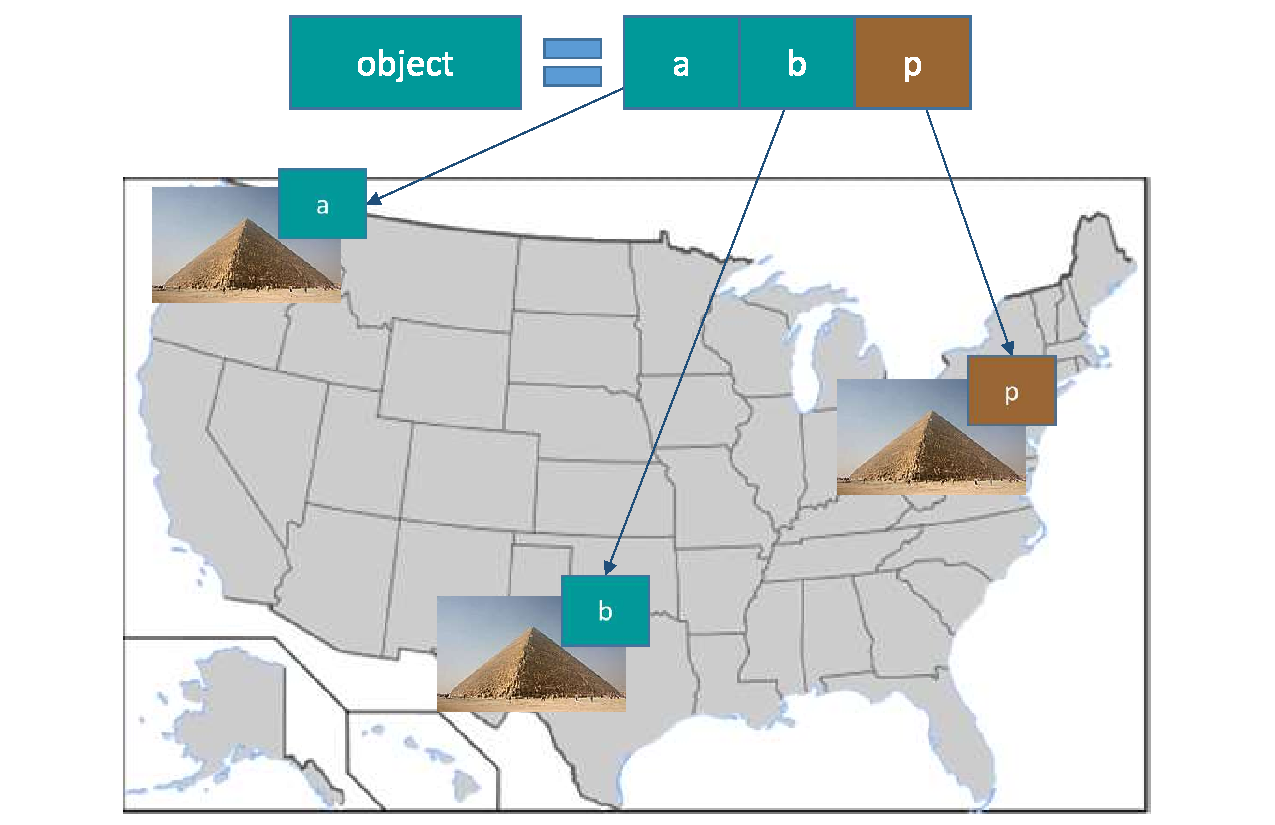
\includegraphics[width=0.4\textwidth]{images/giza_example_crop_fit}
\caption{Storing Object in Giza}
\label{fig:giza_example}
\end{figure}

\subsection{Giza Overview}

Giza exploits the reduction in cross-DC bandwidth cost and leverages erasure coding to optimize the total cost of storing customer data in the cloud. It offers an externally strong consistent (linearizable~\cite{herlihy90linearizability}), versioned object store that erasure codes objects across global data centers.

Customers access Giza by creating Giza storage accounts. For each storage account, the customers have the flexibility to choose the set of data centers where their data are striped across. In addition, they can specify the erasure coding scheme. Giza employs classic $n = k + m$ Reed-Solomon coding, which generates $m$ parity fragments from $k$ data fragments. All $n$ coded fragments are stored in separate DCs, which tolerates up to $m$ arbitrary DC failures.

Figure~\ref{fig:giza_example} illustrates an exemplary flow of storing an object in Giza with 2 + 1 erasure coding. Giza divides the object into two data fragments ($a$ and $b$) and encodes a parity fragment $p$. It then stores the coded fragments in $3$ separate data centers. 

Giza is accessible via {\em put}, {\em get}, and {\em delete} interface. In addition, Giza supports versioning. Each new {\em put} does not overwrite existing data, but rather creates a new version of the data. The old versions remain available until explicitly deleted.

\subsection{Challenges and Contributions}

Giza stripes objects across multiple data centers, so reads and writes require cross-DC communication. The latency is minimized when reads and writes complete with single cross-DC round trips. This is not difficult to achieve for typical Giza workloads, where objects are updated infrequently.

Nevertheless, concurrent updates of the same object do exist. Giza needs to ensure strong consistency when they actually occur. This becomes particularly interesting as Giza allows requests to originate from any DC. Consider two concurrent {\em put} requests of the same object (with different data) from two separate data centers. Depending on network latency, the individual requests may arrive at different data centers in conflicting order. If not handled properly, they would result in data inconsistency. 

To ensure strong consistency, one possible approach is to dedicate a primary data center that handles all requests and enforces execution order. This is less than ideal because the requests from secondary data centers have to be sent to the primary first. This would incur extra cross-DC latency, even when there are no concurrent updates.

Ideally, Giza should optimize for the common case, where reads and writes complete with single cross-DC round trip and achieve minimum latency. This should be true for all reads and writes from any data center. In addition, Giza should ensure consistency in the rare case, where concurrent updates to the same object do occur. It is expected and acceptable that latency would increase as it takes multiple cross-DC round trips to resolve conflict.

%\comment{
%Giza operates on top of existing cloud storage systems. 
%The blob and table storage within individual data centers operate independently.
%Hence, while strongly consistent individually, the collection of the blob and
%table storage across multiple data centers do not readily offer the desired
%external strong consistency. The key technical challenge Giza addresses is how to achieve
%optimal latency with single {\em put}, while at the same time provide
%strong consistency under concurrency, over the collection of individual blob and
%table storages across multiple data centers.
%}

This paper addresses the above key technical challenge and makes the following contributions:
\begin{itemize}
    \item We have designed and implemented Giza, a strongly consistent,
      versioned object store that erasure codes objects across globally
      distributed data centers.
    \item Giza is fast in the common case: when there is no concurrency, Giza
      completes within a single cross-DC round trip, which is optimal given the
      requirement to tolerate data center failure.
    \item Giza ensures strong consistency when accessed concurrently, even with data center
      failure.
    \item Giza adapts well-known distributed algorithms - Paxos~\cite{lamport01paxos}
      and Fast Paxos~\cite{lamport05fast} - in a novel way on top of existing cloud storage systems.
    \item Giza is deployed in \deployment. Experimental results demonstrate
      that Giza achieves our design goals. %In particular, it is worth
      %pointing out that Giza achieves much lower latency than naively adopting a
      %globally consistent storage system, like CockroachDB (widely considered as open source
      %implementation of Google's Spanner).
\end{itemize}
